\documentclass[11pt]{article}
%Gummi|061|=)
\usepackage[table]{xcolor} 
\usepackage{vmargin}
\usepackage[T1]{fontenc} %encoding del font
\usepackage[utf8]{inputenc} %encoding dell'input
\usepackage[italian]{babel} %lingua per la formattazione
\usepackage{mparhack}
\usepackage{pgfplotstable}
\usepackage{float}
%pacchetti per la formattazione
\usepackage{calc} %fantasmi

\usepackage{graphicx} %inserire immagini (grafici vettoriali.pdf)
%pacchetti -->\SCfigure \SCtable
\usepackage{booktabs} %pacchetto per per le tabelle
\usepackage{amsmath, amssymb} %pacchetti per usare comandi matematici
\usepackage{pgf,tikz}
\usepackage{caption}
\usepackage{siunitx}
\usepackage{setspace}
\usepackage{subfig}
\usepackage{array}
\usepackage{multirow}

%\title{\textbf{Equazione di stato dei Gas}\\ %Autori}\author{ xxxxxxxxxxxxx\and
	%	xxxxxxxxxxxxx\and
	%	xxxxxxxxxxxxx}
%\date{\today}
%\setmarginsrb{30mm}{10mm}{20mm}{10mm}
             %{0mm}{10mm}{0mm}{10mm}

%\newcommand{\HRule}{\rule{\linewidth}{0.5mm}}
             
\begin{document}

\begin{center}

% Upper part of the page. The '~' is needed because \\
% only works if a paragraph has started.
% \includegraphics[width=0.20\textwidth]{./Logo1}~\\[1cm]

%\textsc{\LARGE University of Trento}\\[1.5cm]

\textsc{\Huge Esperienza III}\\[0.5cm]
%\vspace{30pt}

%\HRule \\[0.4cm]
%\vspace{15pt}
%{ \huge \bfseries Svuotamento di un volume}\\[0.4cm]
%\vspace{15pt}
%\HRule \\[1.5cm]
%\vspace{30pt}
% Author and supervisor


\large
\title{ESPERIENZA 3}

%\emph{\large\textbf{Autori}}\\ \\ 
Michele \textsc{Pedrotti}\\
Luigi \textsc{Bassini}\\
Nicola \textsc{Trevisson}\\
Giacomo \textsc{Alberini}\\
\vspace{1 cm}
\today





\end{center}

%\tableofcontents

\rowcolors{1}{gray!25}{white}
~\\
%\textbf{Introduzione}\\\\
\section{Montaggio dell'impianto a vuoto}
La prima parte dell'esperienza consisteva nel collegare tra loro un serbatoio di volume, una pompa turbomolecolare, una pompa rotativa, due vacuometri Pirani, un vacuometro a ionizzazione a catodo caldo e un vacuometro a ionizzazione a catodo freddo. 
La difficoltà principale consisteva nel trattare la pompa turbomolecolare nella maniera corretta. Questo tipo di pompa, infatti, può essere accesa solamente quando nella camera è stata raggiunta una pressione di al massimo $10^{-2}$ mbar.
Se la pompa venisse accesa quando la pressione nella camera fosse maggiore, il motore brucerebbe nel tentativo di raggiungere la frequenza di regime. Inoltre, una volta accesa la pompa, la frequenza di rotazione delle pale raggiunge un valore di $9\cdot10^{4}$ giri al minuto. Ne segue che una volta raggiunto il pieno regime, sono necessari diversi minuti prima che, spenta la pompa, le pale cessino di ruotare. 


 \hspace*{0.1mm}Una prima soluzione sarebbe quella di collegare in serie pompa rotativa, pompa turbo molecolare e camera. In questo modo la pompa rotazionale avrebbe portato all'interno della camera un vuoto tale da poter accendere la pompa turbomolecolare, che avrebbe quindi permesso di raggiungere una situazione di Highvacuum. 
\\Questa soluzione, però, non ci avrebbe permesso di riportare la camera alla pressione atmosferica senza dover spegnere la pompa turbomolecolare (e di conseguenza aspettare il tempo necessario all'arresto delle pale).
  
 
 \hspace*{0.1mm}Abbiamo quindi deciso di inserire un raccordo a T in uscita dalla pompa rotazionale, in modo tale da collegare (oltre al sistema in serie) direttamente pompa rotazionale e camera. Questo sistema (oltre all'ausilio delle necessarie valvole) ci permette di riportare la pressione atmosferica nella camera senza dover nè spegnere nè bruciare la pompa turbomolecolare. Riportiamo in figura lo schema da noi adottato.
 \begin{center} 
\begin{figure}[H]
\hspace{-77.5pt}
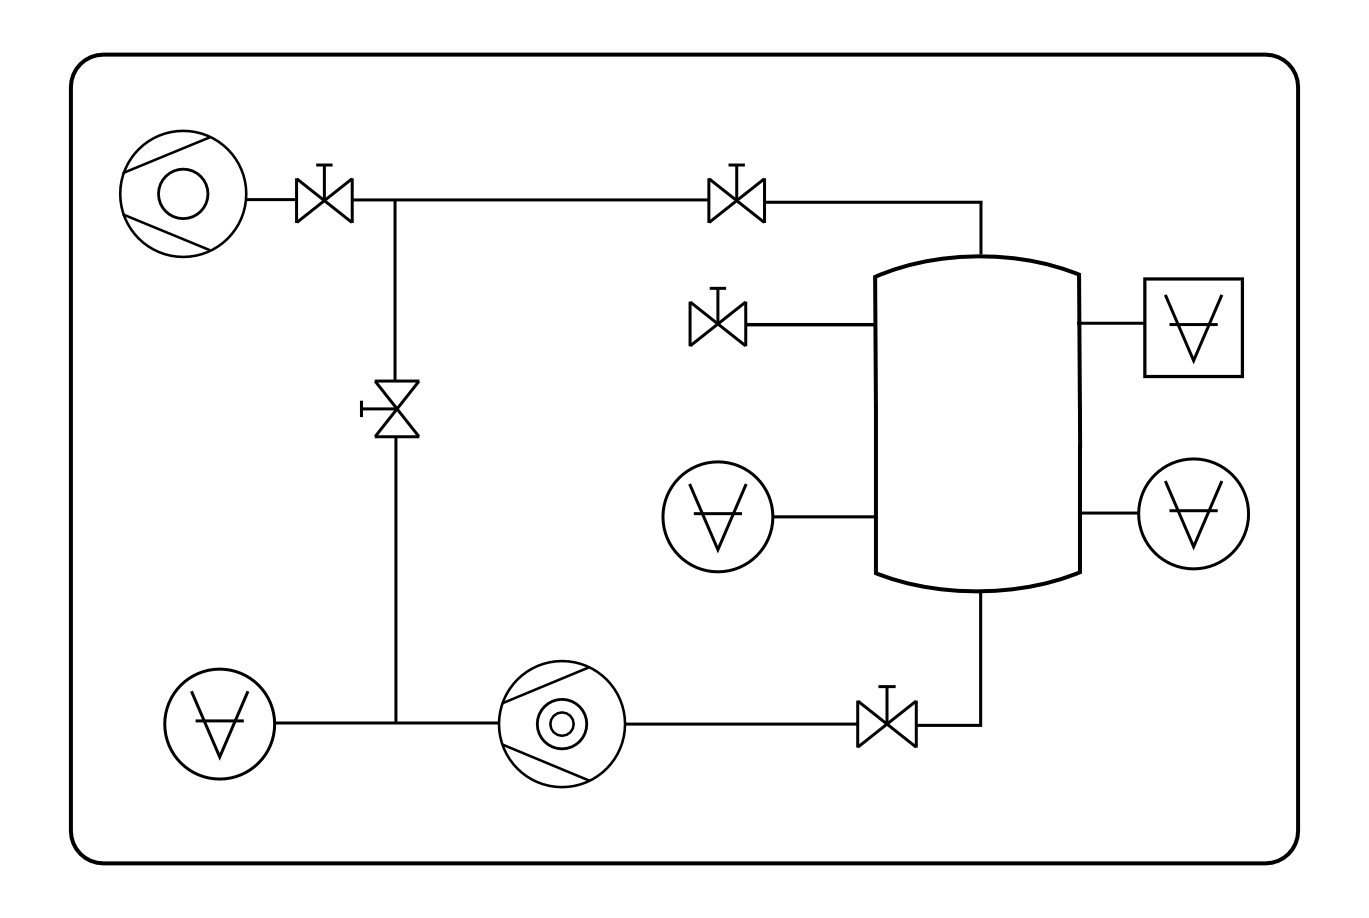
\includegraphics[scale=0.5]{schema_finale.png}
\caption{}
\label{}
\end{figure}
\end{center}

  \hspace*{5mm}Nello schema riportato compaiono quattro vacuometri: due vacuometri Pirani, un vacuometro a catodo caldo e un vacuometro a catodo freddo. I vacuometri hanno l'ovvia funzione di misurare la pressione in diversi punti dell'impianto e con diverse scale di precisione. In particolare i vacuometri Pirani hanno un range di funzionamento compreso tra pressione atmosferica e $10^{-4}$ mbar. Come rappresentato nello schema abbiamo inserito i due Pirani prima e dopo la pompa turbomolecolare. In questo modo siamo riusciti a monitorare la pressione in entrata e in uscita, controllandone il corretto funzionamento. Inoltre il Pirani monitorante la pressione all'interno della camera ci ha permesso di capire quando poter accendere gli altri due vacuometri (a catodo freddo, e a catodo caldo). Questi, infatti, hanno un range di funzionamento compreso tra $10^{-2}$ mbar e $10^{-6}$ mbar (catodo freddo), $10^{-3}$ mbar e $10^{-10}$ mbar (catodo caldo), e se portati fuori scala nel limite superiore possono subire danni anche gravi. Grazie all'utilizzo sequenziale dei diversi vacuometri siamo riusciti a monitorare l'andamento della pressione in camera fino a raggiungere valori di pressioni limite. Questo valore si stabilizzava alla pressione di $1.2\cdot10^{-5}$ mbar.
\section{Taratura vacuometri Pirani}
I vacuometri Pirani devono essere tarati ogni qual volta viene cambiato il gas di cui si intende monitorare la pressione, o comunque dopo ogni utilizzo prolungato. Per tarare questi vacuometri è necessario portare il sensore oltre il range inferiore di lettura, e regolare due trimmer in modo che la tensione passante a pressioni inferiori a $10^{-4}$ mbar sia di 2V. Successivamente è necessario portare il sensore alla pressione atmosferica e, sempre lavorando sui trimmer, regolare la tensione a 10V (è proprio in questo passaggio che si è resa necessaria la presenza del bypass tra la pompa rotazionale e la camera). Questo processo dovrebbe essere ripetuto più volte, in modo da spostare gradualmente la scala verso la taratura desiderata. Nel nostro caso, per limiti di tempo, il processo è stato ripetuto solamente due volte.  

\end{document} 